\chapter{PODSUMOWANIE I WNIOSKI KOŃCOWE}

Opracowane rozwiązanie okazało się niewystarczające. Pomimo spełniania teoretycznych założeń, w praktyce opracowany czujnik nie spełnia swojej funkcji. Wpływa na to parę czynników.

\begin{itemize}
    \item Czujnik przy dużych prędkościach przerywa pomiar, traci orientację w przestrzeni.
    \item Przewody łączące sensor SEN0142 z płytką Arduino wprowadzają dodatkowe zaburzenia:
    \begin{itemize}
        \item są to elementy posiadające masę, dodają więc dodatkowe obciążenie do układu, co przekłada się na zmiany momentów bezwładności elementu obrotowego silnika krokowego,
        \item przewody nie są trwale przyłączone (przylutowane, bądź zaciśnięte rurką termokurczliwą) do modułu SEN0142, nałożono jedynie złącza żeńskie na piny, może więc dochodzić do spadków napięcia, co zaburza prawidłową pracę czujnika.
    \end{itemize}
    \item Ograniczenie częstotliwości próbkowania do $100$ Hz niekorzystnie wpływa na jakość samego pomiaru.
    \item Silnik krokowy jest rozwiązaniem tymczasowym, ponieważ wymusza długi czas symulacji wykonywanej przez LCT. Rozważa się zastosowanie silnika rezonansowego, lub też skanera galwanometrycznego, które docelowo mają skrócić symulację. Czujnik, przez częstotliwość, na której pracuje, nie znajdzie zastosowania w owej technologii (jest zbyt ograniczony).
    \item Opracowane rozwiązanie miałoby zastosowanie przy badaniu obiektów powolnie zmieniających swoje położenie w przestrzeni. Przy prędkościach z jakimi porusza się silnik krokowy, czujnik obecnie nie jest przydatny.
\end{itemize}

Kolejnym ograniczającym rozwiązaniem było wykorzystanie \emph{Microsoft WPF}. Pomimo, że umożliwia łatwe i szybkie utworzenie aplikacji z graficznym interfejsem, blokuje ono wykorzystanie programu na innych systemach operacyjnych niż \emph{Microsoft Windows}. Jeśli aplikacja miałaby być multiplatformowa (potencjalnie z implementacją również na urządzeniach mobilnych) warto by było zastosować platformę do stworzenia aplikacji webowej (np. React.JS, Angular, Google Flutter), dzięki czemu zostałoby zniwelowane ograniczenie do jednej platformy. Co więcej, przy integracji z bazą danych, możliwe by było jednoczesne składowanie wcześniej wykonanych pomiarów.

Należałoby również wymienić moduł na taki, który posiada wbudowany przekaźnik bezprzewodowy. Zniwelowałoby to problem jakim są przewody, a raczej ich masa. Jednakże, w takim wypadku trzeba zagwarantować jak najmniejszą stratę danych.

Rozwiązaniem, które umożliwiłoby pracę czujnika na większych częstotliwościach, wymagałoby wykorzystania pamięci Arduino - skrypt zapisywałby pomiary na płytce, a dopiero potem przesyłał je do komputera. Byłoby to problematyczne o tyle, że tej jest relatywnie niewiele. Należałoby zastosować rozwiązanie technologiczne umożliwiające podłączenie dodatkowej pamięci, np. Raspberry Pi. Byłoby ono o tyle wygodne, że w odróżnieniu od Arduino, które jest jedynie płytką z mikrokontrolerem, jest to w pełni funkcjonalny komputer, z własnym systemem operacyjnym na jądrze Linuxa. Takie rozwiązanie byłoby rozsądniejsze o tyle, że samą aplikację sterującą można by zaimplementować już na Raspberry Pi. Dodatkowym atutem jest łatwiejsze programowanie - to bazuje na Bashu lub Pythonie.

\begin{figure}[H]
    \centering
    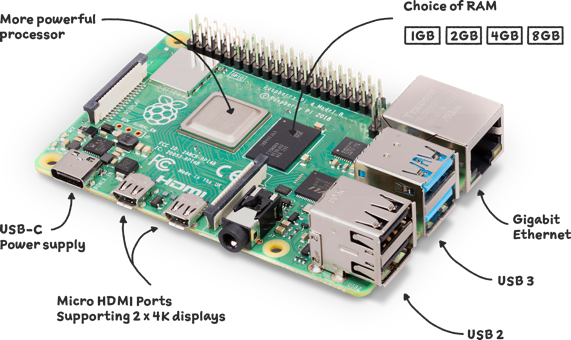
\includegraphics[width=\textwidth]{pictures/raspberry_pi_4.png}
    \caption{Komputer Raspberry Pi 4B \cite{pi}}
    \label{fig:rsp}
\end{figure}

Na rys. 5.1 widać, że zniknąłby problem z prędkością przesyłania danych, bo te byłyby bezpośrednio składowane na Raspberry Pi, lub też pamięci zewnętrznej podłączonej do tego komputera. Samo urządzenie ma wbudowane złącze Ethernet (dostęp do internetu w razie potrzeby jest więc zapewniony). Można je również skonfigurować z mocniejszym komputerem by działały w relacji master-slave. Wadą tego rozwiązania jest jednak cena zestawu - na przestrzeni ostatnich lat Raspberry Pi podrożało, gdyż zaczęto je wykorzystywać do kopania kryptowalut.

